Dans les chapitres précédents, nous avons vu comment résoudre des problèmes de recherche. 
Dans ce chapitre, nous allons nous concentrer sur les problèmes où nous devons \textbf{battre nos adversaire} 
dans des jeux à \textbf{deux ou plusieurs joueurs}.

\subsection{Définition d'un jeu} % (fold)
\label{sub:definition_d_un_jeu}

\begin{definition}{Jeu}{game}
    Un jeu est un problème de recherche avec les caractéristiques suivantes:
    \begin{itemize}
        \item \textbf{État initial, $s_0$}: la position initiale du jeu.
        \item \textbf{Joueur, $Player(s)$}: le joueur qui doit jouer.
        \item \textbf{Actions, $Action(s)$}: les coups possibles pour un joueur.
        \item \textbf{Modèle de transition, $Result(a, s)$}: L'état $s'$ qui résulte de l'action $a$ dans l'état $s$
        \item \textbf{Fonction de terminal, $isTerminal(s)$}: la fonction qui détermine si le jeu est terminé
        \item \textbf{Utilité, $Utility(s, p)$}: la fonction qui détermine le score du jeu sur les états terminaux. Qui gagne,et combien.
            $p$ est le joueur.
    \end{itemize} 
\end{definition}
\begin{note}
    Il y a plusieurs types de jeux:
    \begin{itemize}
        \item \textbf{Jeux à somme nulle}: la somme des utilités des joueurs est toujours égale à 0. Si l'un \textbf{gagne}, l'autre \textbf{perd}.
        \item \textbf{Jeux à somme général}: Les agents peuvent avoir des utilités différentes. Si l'un \textbf{gagne}, l'autre \textbf{ne perd pas forcément}. (\textit{Coop}, \textit{...})
        \item \textbf{Jeux d'équipes}: Les agents jouent en équipe contre d'autres agents.
    \end{itemize}
\end{note}
% subsection Definition d'un jeu (end)

\subsection{Minimax} % (fold)
\label{sub:minimax}

\begin{definition}{Minimax}{minimax}
    L'algorithme \textbf{Minimax} est un algorithme qui permet de trouver le meilleur coup à jouer dans un jeu \textbf{déterministe} à \textbf{somme nulle}.
    Le principe est simple, nous imaginons 2 joueurs qui jouent l'un contre l'autre, \textbf{Min} et \textbf{Max}.
    Le but de \textbf{Max} est de maximiser l'utilité et le but de \textbf{Min} est de minimiser l'utilité sachant 
    que l'autre joueur va jouer de manière optimale.
\end{definition}

\begin{figure}[H]
    \begin{center}
        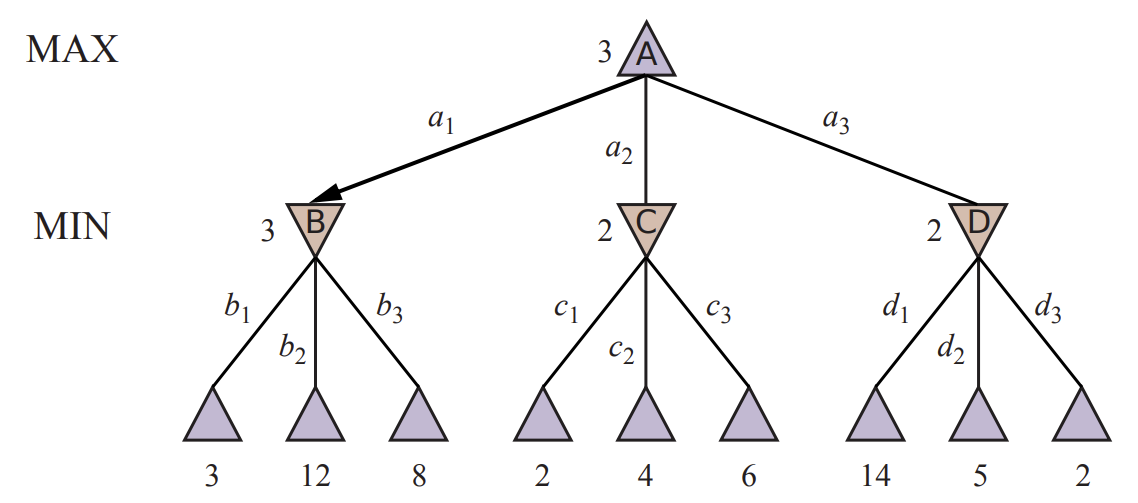
\includegraphics[width=0.55\textwidth]{./pictures/minimax.png}
    \end{center}
    \caption{Minimax dans un arbre}\label{fig:minimaxtree}
\end{figure}

\begin{algorithm}[H]
    \floatname{algorithm}{Minimax}
    \caption{Algorithme Minimax}\label{alg:minimax}
    \begin{algorithmic}
        \Function{Minimax-Search}{game, state} 
        \State player $\leftarrow$ game.\Call{To-Move}{state}
        
        \If{player = max}
            \State value, action $\leftarrow$ \Call{Max-Value}{game, state} 
        \Else 
            \State value, action $\leftarrow$ \Call{Min-Value}{game, state}
        \EndIf
        \State \Return action
        \EndFunction
        \vspace{0.5cm}
        \Function{Max-Value}{game, state}
        \If{game.\Call{Terminal-Test}{ state}}
            \State \Return game.\Call{Utility}{state, player}, $null$
        \EndIf 
        \State value, action $\leftarrow -\infty, null$

        \For{action in game.\Call{Actions}{state}}
            \State value2, action2 $\leftarrow$ \Call{Min-Value}{game, game.\Call{Result}{state, action}}
            \If{value2 $>$ value}
                \State value, action $\leftarrow$ value2, action2
            \EndIf
        \EndFor

        \Return value, action
        \EndFunction
        \vspace{0.5cm}
        \Function{Min-Value}{game, state} 
        \If{game.\Call{Terminal-Test}{ state}}
            \State \Return game.\Call{Utility}{state, player}, $null$
        \EndIf 
        \State value, action $\leftarrow \infty, null$ 

        \For{action in game.\Call{Actions}{state}}
        \State value2, action2 $\leftarrow$ \Call{Max-Value}{game, game.\Call{Result}{state, action}}%{game, game.\Call{Result}{state, action}}
            \If{value2 $<$ value}
                \State value, action $\leftarrow$ value2, action2 
            \EndIf
        % }
        \EndFor
        \State \Return value, action
        \EndFunction
    \end{algorithmic} 
\end{algorithm}

L'algorithme va généré l'arbre de recherche jusqu'aux étas \textbf{terminaux} pour utiliser la fonction d'utilité. 
Il traite ensuite ces valeurs en remontant l'arbre et les choisit en fonction du joueur qui doit jouer (\textbf{Min} ou \textbf{Max})
\begin{note}
    Pour ne pas généré tous l'arbre, on peut utiliser une \textbf{profondeur limitée}.
\end{note}

Si il y a plus de 2 joueurs, nous pouvons assigner à chaque noeud un tuple de valeurs qui représente l'utilité pour chaque joueur. 
Chaque joueur va alors choisir le coup qui maximise son utilité. 

\begin{remark}\leavevmode
    Cet algortihme est basé sur \textbf{DFS}. 
    \begin{itemize}
        \item \textbf{Complexité en temps}: $O(b^m)$
        \item \textbf{Complexité en espace}: $O(bm)$
    \end{itemize}
\end{remark}

\begin{figure}
    \begin{center}
        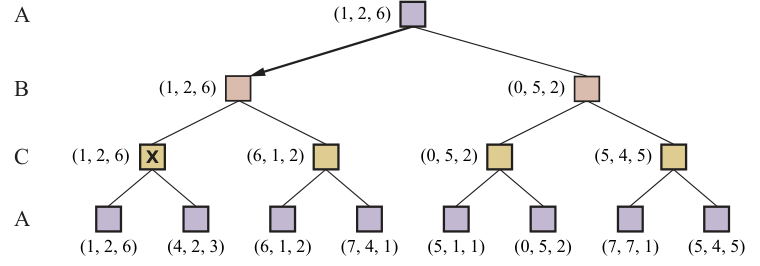
\includegraphics[width=0.65\textwidth]{./pictures/multiminimax.png}
    \end{center}
    \caption{Représentation en Multijoueur}\label{fig:mutliminimax}
\end{figure}
% subsection Minimax (end)

\subsection{Alpha-Beta pruning} % (fold)
\label{sub:alpha_beta_pruning}

\begin{definition}{Alpha-Beta pruning}{alphabeta}
    L'algorithme \textbf{Alpha-Beta pruning} est un algorithme qui permet de trouver le meilleur coup à jouer dans un jeu \textbf{déterministe} à \textbf{somme nulle}.
    Il est basé sur l'algorithme \textbf{Minimax} mais il va \textbf{couper} les branches qui ne sont pas intéressantes.
    Il utilise 2 paramètres, $\alpha$ et $\beta$ qui représentent les valeurs minimales et maximales que l'on peut atteindre.
    \begin{itemize}
        \item $\alpha$ est la meilleure option (valeure la plus haute) que le joueur \textbf{Max} est assuré d'obtenir. 
            \textbf{Au MOINS}.
        \item $\beta$ est la meilleure option (valeure la plus basse) que le joueur \textbf{Min} est assuré d'obtenir. 
            \textbf{Au PLUS}.
    \end{itemize} 
\end{definition}

\begin{remark}\leavevmode
    Le meilleur situation pour cette algorithme est quand les meilleurs coups sont toujours le 
    premier coup à être évalué (\textit{plus à gauche})
\end{remark}

\begin{figure}[H]
    \begin{center}
        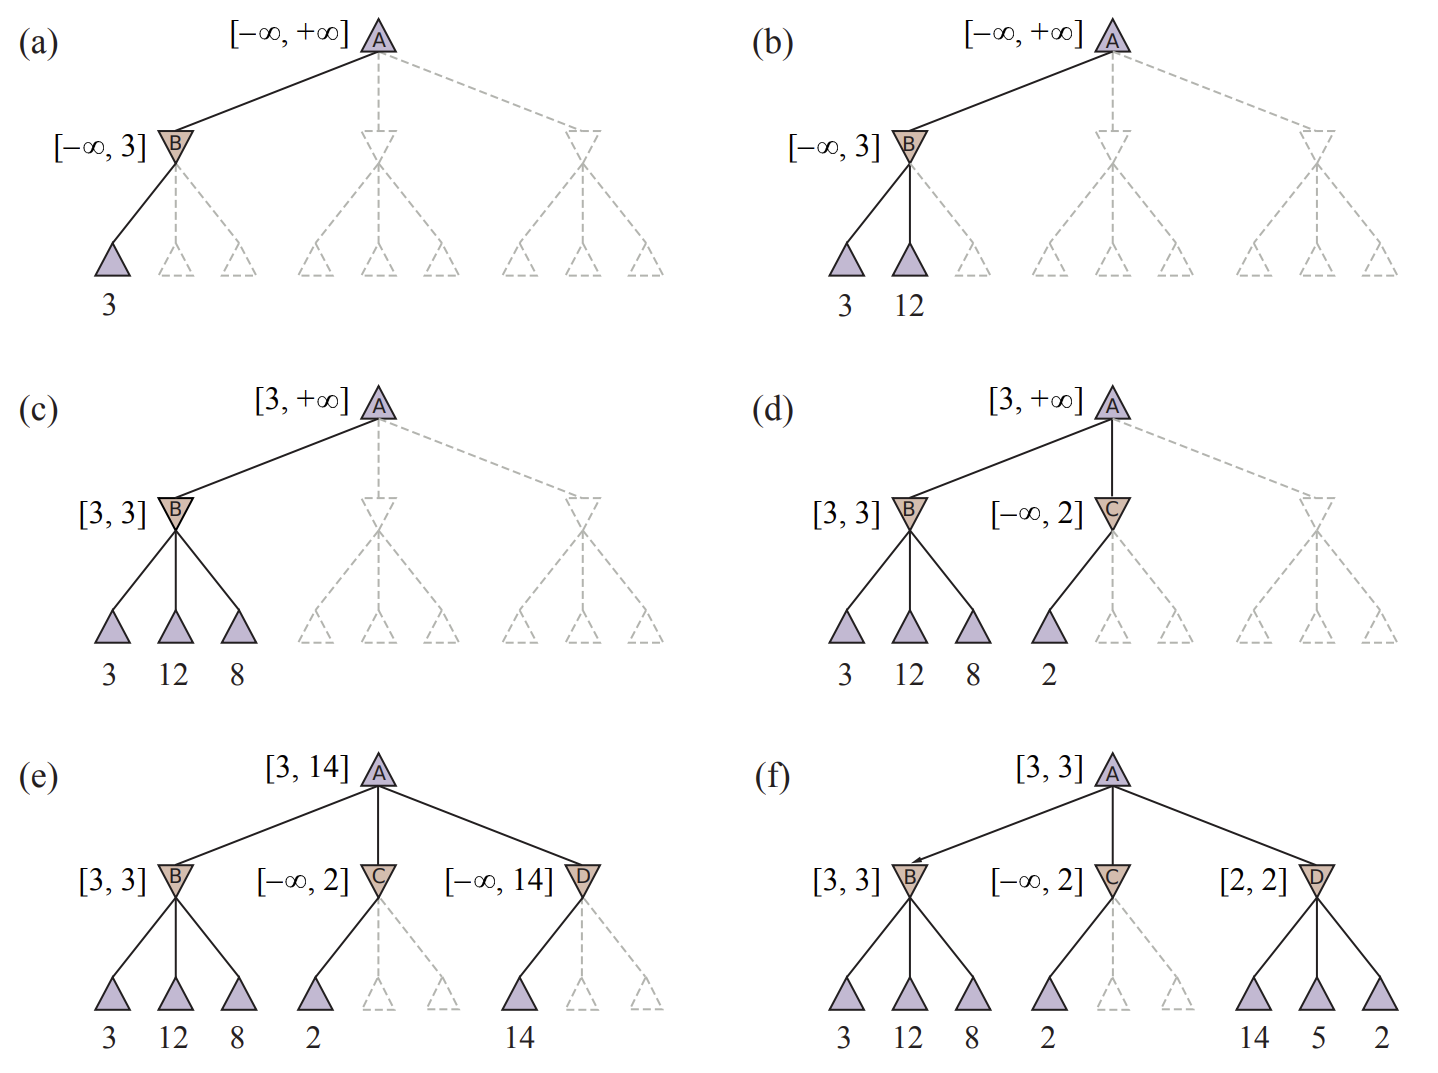
\includegraphics[width=0.65\textwidth]{./pictures/alphabeta.png}
    \end{center}
    \caption{Alpha-Beta pruning dans un arbre}\label{fig:alphabeta} 
\end{figure}

\begin{remark}\leavevmode
    La complexité en temps est généralement plus petite que celle de minimax
    \begin{itemize}
        \item \textbf{Complexité en temps}: $O(b^{m/2})$ avec les noeuds dans le \textbf{bon} ordre
            et $O(b^{3m/4})$ si les noeuds sont visités aléatoirement.
        \item \textbf{Complexité en espace}: $O(bm)$ et $O(\sqrt{b})$ si les noeuds sont dans le bon ordre.
    \end{itemize}
\end{remark}

Si cet algorithme n'est pas suffisant, on peut utilisé une fonction d'évaluation qui permet d'évaluer les noeuds 
qui ne sont pas des états terminaux pour estimer leur utilité.

\scalebox{0.8}{
    \begin{minipage}{\textwidth}
        \centering
        \begin{algorithm}[H]
            \floatname{algorithm}{$\alpha-\beta$ pruning}
            \caption{Algorithme $\alpha-\beta$ pruning}\label{alg:alphabeta}
            \begin{algorithmic}
                \Function{Minimax-Search}{game, state} 
                \State player $\leftarrow$ game.\Call{To-Move}{state}
                \State value, action $\leftarrow$ \Call{Max-Value}{game, state, $-\infty$, $+\infty$}
                \State \Return action
                \EndFunction
                \vspace{0.5cm}

                \Function{Max-Value}{game, state, $\alpha$, $\beta$}
                \If{game.\Call{Terminal-Test}{ state}}
                    \State \Return game.\Call{Utility}{state, player}, $null$
                \EndIf 
                \State value, action $\leftarrow -\infty, null$

                \For{action in game.\Call{Actions}{state}}
                    \State value2, action2 $\leftarrow$ \Call{Min-Value}{game, game.\Call{Result}{state, action}, $\alpha$, $\beta$}
                    \If{value2 $>$ value}
                        \State value, action $\leftarrow$ value2, action2
                        \State $\alpha \leftarrow$ \Call{Max}{$\alpha$, value}
                    \EndIf
                    \If{$v \geq \beta$}
                        \State \Return value, action 
                    \EndIf
                \EndFor
                \Return value, action
                \EndFunction

                \vspace{0.5cm}
                \Function{Min-Value}{game, state, $\alpha$, $\beta$}
                \If{game.\Call{Terminal-Test}{ state}}
                    \State \Return game.\Call{Utility}{state, player}, $null$
                \EndIf 
                \State value, action $\leftarrow \infty, null$ 

                \For{action in game.\Call{Actions}{state}}
                \State value2, action2 $\leftarrow$ \Call{Max-Value}{game, game.\Call{Result}{state, action}, $\alpha$, $\beta$}
                    \If{value2 $<$ value}
                        \State value, action $\leftarrow$ value2, action2 
                        \State $\beta \leftarrow$ \Call{Min}{$\beta$, value}
                    \EndIf
                    \If{$v \leq \alpha$}
                        \State \Return value, action 
                    \EndIf
                \EndFor
                \State \Return value, action
                \EndFunction
            \end{algorithmic} 
        \end{algorithm}
    \end{minipage}
}

% subsection Alpha-Beta pruning (end)
